\documentclass[thesis.tex]{subfiles}
\begin{document}

\chapter{SpeedCam}\label{chap:basics}

The REAL stuff. All your precious work written down for the benefit of humanity.

\section{Overview}

\section{Detection scheme}
This part will contain the description about the detection scheme. It will outline how to detect a greedy user and provide a detailed overview of its functionality.

\subsection{Basic idea}
The task of the detection scheme is to identify a greedy AS inside an ISD using multi-path connections. 

A central unit inside the ISD will be able to start an inspection and inspect ASes bandwidth usage. This is done by a core AS, which is called \textbf{inspector}. 

The inspector will randomly choose ASes inside its ISD to measure the bandwidth. The chosen ASes are called \textbf{speed cam}. They will collect for a certain amount of time the metrics and aggregate them over time. When the duration is to end, the speed cams will sent the data to the inspector.

When the inspector received the data of all speed cams, he will decide, which user is greedy and who are not. The decision process will be explained in later parts of this work.


\begin{figure}[h]
    \begin{subfigure}{.32\linewidth}
        \centering
        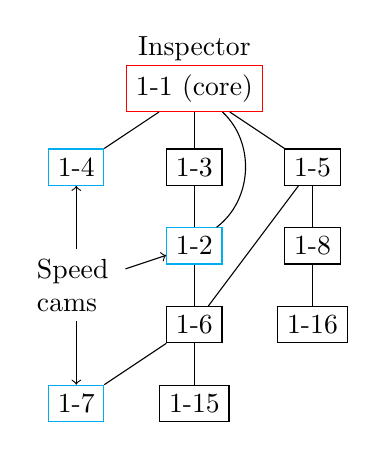
\begin{tikzpicture}
        \node (inspector) at (0, 0.5) {Inspector};
        \node[shape=rectangle,draw=red] (1-1) at (0,0) {1-1 (core)};
        \node[shape=rectangle,draw=cyan] (1-2) at (0,-2) {1-2};
        \node[shape=rectangle,draw=black] (1-3) at (0,-1) {1-3};
        \node[shape=rectangle,draw=cyan] (1-4) at (-1.5,-1) {1-4};
        \node[shape=rectangle,draw=black] (1-5) at (1.5,-1) {1-5};
        \node[shape=rectangle,draw=black] (1-6) at (0,-3) {1-6};
        \node[shape=rectangle,draw=cyan] (1-7) at (-1.5,-4) {1-7};
        \node[shape=rectangle,draw=black] (1-8) at (1.5,-2) {1-8};
        \node[shape=rectangle,draw=black] (1-15) at (0,-4) {1-15};
        \node[shape=rectangle,draw=black] (1-16) at (1.5,-3) {1-16};
        \node (speedcam) at (-1.5, -2.5) [text width=1cm]{Speed cams};        
        
        \path[-]	
        (1-1) edge (1-4)
        (1-1) edge (1-3)
        (1-1) edge (1-5)
        (1-1) edge[bend left=50] (1-2)
        (1-2) edge (1-6)
        (1-3) edge (1-2)
        (1-5) edge (1-8)
        (1-5) edge (1-6)
        (1-6) edge (1-7)
        (1-6) edge (1-15)
        (1-8) edge (1-16)
        ;
        
        \path[->]
        (speedcam) edge (1-4)
        (speedcam) edge (1-2)
        (speedcam) edge (1-7);
        \end{tikzpicture}
        \caption{Inspector choose ASes for speed cams}
        \label{fig:main:exampleDetectionSchemeSub1}
    \end{subfigure}%
    \begin{subfigure}{.32\linewidth}
        \centering
        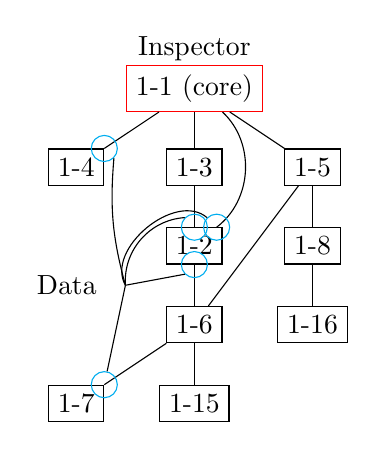
\begin{tikzpicture}
        \node (inspector) at (0, 0.5) {Inspector};
        \node[shape=rectangle,draw=red] (1-1) at (0,0) {1-1 (core)};
        \node[shape=rectangle,draw=black] (1-2) at (0,-2) {1-2};
        \node[shape=rectangle,draw=black] (1-3) at (0,-1) {1-3};
        \node[shape=rectangle,draw=black] (1-4) at (-1.5,-1) {1-4};
        \node[shape=rectangle,draw=black] (1-5) at (1.5,-1) {1-5};
        \node[shape=rectangle,draw=black] (1-6) at (0,-3) {1-6};
        \node[shape=rectangle,draw=black] (1-7) at (-1.5,-4) {1-7};
        \node[shape=rectangle,draw=black] (1-8) at (1.5,-2) {1-8};
        \node[shape=rectangle,draw=black] (1-15) at (0,-4) {1-15};
        \node[shape=rectangle,draw=black] (1-16) at (1.5,-3) {1-16};
        \node (data) at (-1.5, -2.5) [text width=1cm]{Data};
        
        \path[-]		
        (1-1) edge node[shape=circle,draw=cyan, at end] (data1) {} (1-4)    
        (1-1) edge (1-3)
        (1-1) edge (1-5)
        (1-1) edge[bend left=50] node[shape=circle,draw=cyan, at end] (data2) {} (1-2)
        (1-2) edge node[shape=circle,draw=cyan, at start] (data3) {} (1-6)
        (1-3) edge node[shape=circle,draw=cyan, at end] (data4) {} (1-2)
        (1-5) edge (1-8)
        (1-5) edge (1-6)
        (1-6) edge node[shape=circle,draw=cyan, at end] (data5) {} (1-7)
        (1-6) edge (1-15)
        (1-8) edge (1-16)
        ;
        \path[-]
        (data1.south east) edge[bend right=10] (data.east)
        (data2.north west) edge[bend right=80] (data.east)
        (data3.south west) edge (data.east)
        (data4.north west) edge[bend right=45] (data.east)
        (data5) edge (data.east)
        ;
        \end{tikzpicture}
        \caption{Speed cams collect data about traffic}
        \label{fig:main:exampleDetectionSchemeSub2}
    \end{subfigure}%
    \begin{subfigure}{0.32\linewidth}
        \centering
        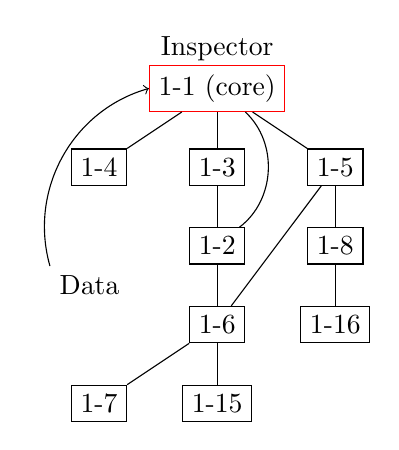
\begin{tikzpicture}
        \node (inspector) at (0, 0.5) {Inspector};
        \node[shape=rectangle,draw=red] (1-1) at (0,0) {1-1 (core)};
        \node[shape=rectangle,draw=black] (1-2) at (0,-2) {1-2};
        \node[shape=rectangle,draw=black] (1-3) at (0,-1) {1-3};
        \node[shape=rectangle,draw=black] (1-4) at (-1.5,-1) {1-4};
        \node[shape=rectangle,draw=black] (1-5) at (1.5,-1) {1-5};
        \node[shape=rectangle,draw=black] (1-6) at (0,-3) {1-6};
        \node[shape=rectangle,draw=black] (1-7) at (-1.5,-4) {1-7};
        \node[shape=rectangle,draw=black] (1-8) at (1.5,-2) {1-8};
        \node[shape=rectangle,draw=black] (1-15) at (0,-4) {1-15};
        \node[shape=rectangle,draw=black] (1-16) at (1.5,-3) {1-16};
        \node (data) at (-1.5, -2.5) [text width=1cm]{Data};
        
        \path[-]	
        (1-1) edge (1-4) 
        (1-1) edge (1-3)
        (1-1) edge (1-5)
        (1-1) edge[bend left=50] (1-2)
        (1-2) edge (1-6)
        (1-3) edge (1-2)
        (1-5) edge (1-8)
        (1-5) edge (1-6)
        (1-6) edge (1-7)
        (1-6) edge (1-15)
        (1-8) edge (1-16)
        ;
        
        \path[->]
        (data.north west) edge[bend left=45] (1-1.west);
        \end{tikzpicture}
        \caption{Speed cams report data to inspector}
        \label{fig:main:exampleDetectionSchemeSub3}
    \end{subfigure}
    \caption{Example of detection scheme}
    \label{fig:main:exampleDetectionScheme}
\end{figure}

The \autoref{fig:main:exampleDetectionScheme} shows an example for the detection scheme. It shows a the ISD 1 and its ASes. In \autoref{fig:main:exampleDetectionSchemeSub1} is the process of choosing speed cams visualized. The ASes 1-2, 1-4 and 1-7 are randomly chosen and now called speed cams. For a certain amount of time, the speed cams collect data about traffic through their border router. This can be seen in \autoref{fig:main:exampleDetectionSchemeSub2}. After the collection is finished, the data is sent to the inspector, which is shown by \autoref{fig:main:exampleDetectionSchemeSub3}.

The following section will explain the details about the selection, the data to collect and to classify the user.

\subsection{Selection process}
This part will explain the process how ASes are selected to be speed cams.

It is obvious that the inspector has to randomly pick ASes at random time slots. If the process were deterministic, then malicious ASes could exploit it. They would use fewer resources at the time of the inspection and so avoid punishment.

It is also important to only inspect, when it is necessary. By limiting the monitoring, fewer resources as the bandwidth or computation time are utilized. One possibility is to start the inspection when a bandwidth is exceeded inside the ISD. This happens when the total currently used bandwidth of a connection is higher than the capacity. Using the method can be too late to avoid the congestion, but it would limit the resource usage. 
It is also important to have a cooldown time between inspection, even if the congestion cannot be solved by punishing greedy user. Otherwise the inspection will be done without an effect.

\todo{Add example graph for that}

Another approach is to prevent such data jams by randomly monitoring ASes throughout the day. This would be done without the urgent need of a bandwidth exceed. This will waste resources but can identify a greedy user before he can disturb other user. 

A mix of both approaches will be investigated by this work. The first investigation will be shorter than the second because of the urgency to identify the source of the congestion. The second one can be done over a longer period for a more accurate result.

\todo{Add obvious impossible approaches: ALways monitor, never monitor}

The necessary amount of speed cams inside a ISD is one interesting question to answer. Fewer speed cams result in a lower resource impact, which is good. But it will also result in a lower precision, which can lead to wrong accusations or missing greedy users.

A pure random amount of ASes is a intuitive answer, but in big ISD with hundreds of ASes only one speed cam will be not enough to measure multi-path bandwidth. An improved version is that the amount is between a certain percentage of the total ASes and the total number itself.

\todo{This should be answered inside experiments or maybe in further works?}

\subsection{Data and metrics}
This part will describe the metrics which are measured and the resulting data which is collected by the inspection.

Each speed cam will collect the same data over the same time period and sent them to the inspector. The data will be aggregated over time, if possible, to minimize the memory consumption of the ASes.

The following list show this metrics:
\begin{easylist}
    \MyListProperties
    # avg. bandwidth usage per AS
    # avg. sent packets per AS
    # avg. received packets per AS
    # requests to path server 
\end{easylist}

The requests to the path server can be used to find the different path an AS uses for its transmissions. 

It is also necessary that the inspector has the complete topology of its ISD. This is used to calculate the percentage of available and used bandwidth by an AS. There is currently no central unit which has the complete topology of its ISD. Nevertheless, it is possible to calculate it by fetching the path receive requests from the Path server. 

The data stored in the topology are the following:

\begin{easylist}
    \MyListProperties
    # source AS
    # destination AS
    # bandwidth in bits per second
\end{easylist}
\todo{Rotate clockwise for better page utilization}
\begin{figure}[h]
    \centering
    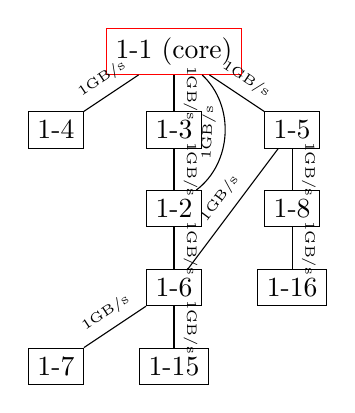
\begin{tikzpicture}
    \node[shape=rectangle,draw=red] (1-1) at (0,0) {1-1 (core)};
    \node[shape=rectangle,draw=black] (1-2) at (0,-2) {1-2};
    \node[shape=rectangle,draw=black] (1-3) at (0,-1) {1-3};
    \node[shape=rectangle,draw=black] (1-4) at (-1.5,-1) {1-4};
    \node[shape=rectangle,draw=black] (1-5) at (1.5,-1) {1-5};
    \node[shape=rectangle,draw=black] (1-6) at (0,-3) {1-6};
    \node[shape=rectangle,draw=black] (1-7) at (-1.5,-4) {1-7};
    \node[shape=rectangle,draw=black] (1-8) at (1.5,-2) {1-8};
    \node[shape=rectangle,draw=black] (1-15) at (0,-4) {1-15};
    \node[shape=rectangle,draw=black] (1-16) at (1.5,-3) {1-16};
    
    \path[-]	
    (1-1) edge node[sloped, anchor=center, above] {\tiny 1GB/s} (1-4) 
    (1-1) edge node[sloped, anchor=center, above] {\tiny 1GB/s} (1-3)
    (1-1) edge node[sloped, anchor=center, above] {\tiny 1GB/s} (1-5)
    (1-1) edge[bend left=50] node[sloped, anchor=center, above] {\tiny 1GB/s} (1-2)
    (1-2) edge node[sloped, anchor=center, above] {\tiny 1GB/s} (1-6)
    (1-3) edge node[sloped, anchor=center, above] {\tiny 1GB/s} (1-2)
    (1-5) edge node[sloped, anchor=center, above] {\tiny 1GB/s} (1-8)
    (1-5) edge node[sloped, anchor=center, above] {\tiny 1GB/s} (1-6)
    (1-6) edge node[sloped, anchor=center, above] {\tiny 1GB/s} (1-7)
    (1-6) edge node[sloped, anchor=center, above] {\tiny 1GB/s} (1-15)
    (1-8) edge node[sloped, anchor=center, above] {\tiny 1GB/s} (1-16)
    ;
    \end{tikzpicture}
    \caption{Example topology with annotated bandwidth}
    \label{fig:main:exampleTopology}
\end{figure}

When a new inspector is implemented inside an ISD, he has to construct the topology by periodically fetch the newest path requests. Because the topology remains static rather than constantly changing, the fetch rate can be high at the beginning and decrease to a normal value. For example, when the inspector is created, the fetch rate is 0.1 second and will decrease to 1.0 second of a few hours. 

\todo{Use work of ? with his buckets to get the values}

\subsection{Classify user}
This part will explain what a greedy user is and how to distinguish between a greedy and a normal user. It contain a definition for this work, which will later be used.

A greedy user is a user, who uses his network resources as the bandwidth in a selfish way and tries to maximize his personal benefit by using as much bandwidth as possible. He even may try to overuses his subscribed bandwidth or avoid the limits by using multi path communication.

An user may also be classified as a more greedy user than a fair user, when here is a congestion in the network and this user uses the most bandwidth. He may not be acting greedy in the first place, but he can be considered greedy in a global view.

Because of this we have to view two aspects which can classify a user as greedy. The first is the use of his resources. He can stay in the limit or he can overuse it. The second is if his activity causes a congestion.
\begin{table}[h]
    \centering
    \begin{tabular}{ r|c|c| }
        \multicolumn{1}{r}{}
        &  \multicolumn{1}{c}{no congestion}
        & \multicolumn{1}{c}{congestion} \\
        \cline{2-3}
        stays in limit & I & II \\
        \cline{2-3}
        overuses limit & III & IV \\
        \cline{2-3}
    \end{tabular}
    \caption{Different cases of a greedy user}
    \label{tab:classifyUser}    
\end{table}

\autoref{tab:classifyUser} shows these different four cases. The stays im limit or overuses limit means only the bandwidth usage of one connection between two ASes. An AS can have multiple connection to different ASes and can stay in his local limits.

\subsubsection{Case I - Fair user} \label{sub:main:detection:case1}
This user uses fewer bandwidth than he has subscribed to. There is also no congestion inside the network. In this case, there is no need to punish the user. They could use even more bandwidth, because it is currently underutilized and wasted.

\subsubsection{Case II - Global greedy user}
In this case there is a congestion inside the network. The currently used bandwidth is higher than the available. But there is no user who uses more bandwidth than he has subscribed to. Because of the missing culprit the punishment is not as easy as in case 4.

There is a need to find the most greedy user and try to convince him to use less resources for a better network experience for every user. The problem is, to find the most greedy user and to distinguish him from other user.

This can be done by using a clustering algorithm to find user with a similar behaviour. The cluster algorithm needs to find the outlier using more bandwidth than other. It also has to perform well with bigger sizes of elements, any $log(n^2)$ or worse runtime complexity is not sufficient. Because of using only the bandwidth as an attribute, it is possible to use algorithm based on arrays or lists of values, which results in simpler and more efficient algorithm.

The algorithm used for this work is the \textit{Jenks Natural Breaks} algorithm. \todo{Add good source}
%, Jenks Natural Breaks: https://www.ehdp.com/vitalnet/breaks-1.htm, http://wiki.objectvision.nl/index.php/Fisher\%27s_Natural_Breaks_Classification
It is applied to a sorted list of values and find good fitting ranges with also a rating value from 0 (worst fit) to 1 (perfect fit). Originally used for creating chloropleth maps, it can be used to divide the amount of users into two groups: fair user and user with high bandwidth usage. 

\todo{Explain the algorithm?}

If the GVF is higher than 0.8 we can assume, that the second range describes user who uses more bandwidth than the other. The member in this range can be considered as more greedy user than the other.


\todo{Add figure to display the issue}

\subsubsection{Case III - Overusing with no congestion}
This case occurs when there is no congestion, but an AS uses more bandwidth than it has subscribed for. For example, an AS has only a subscription for 1 GBit/s, but uses 1.2 GBit/s. The difference to case IV is, that beside overusing, there is no congestion.

On the one hand this behaviour can quickly lead to a congestion when everybody is doing it. On the other hand this behaviour utilizes the bandwidth in a better way, because the wasted bandwidth by not using it is lower.

The user can be clearly considered as greedy, but do not need to be punished immediately. A better way would be to tolerate a certain percentage of overuse and punish the user if he uses more than tolerated. The tolerance range would be 10\% without any problems. If the AS uses more than 110\% of its bandwidth the AS should be considered as a greedy user and receive a delayed punishment.

\todo{Add line graph to visualize this part}

\subsubsection{Case IV - Overuse resulted in a congestion}
This case is much more simpler than the other. If there is a congestion any user who overuses his bandwidth is considered a greedy user and have to receive immediately punishment to reduce or stop the congestion. 

\section{Next parts}
\begin{easylist}
    \MyListProperties
        ## Parameters of detection scheme
        ### Frequency
        ### Duration
        ### Sample size
        ## Security
        ### How to prevent lying AS
        ### How to prevent misusing the system(for dDos)
        # Punishment scheme
        ## Overview
        ## Level system for punishment (\textit{Flensburger system})
        ### \textit{Table of different levels and their punishments}
        ### How to get \"points\"
        ### Explain the levels
        ## Enforcement of punishment
        ### Describe responsibility (coreAS or coordinator?)
    \end{easylist}
\subfilebib % Makes bibliography available when compiling as subfile
\end{document}